\graphicspath{ {./bilder/} }

\subsection{Eulers metode}
Eulers metode er en metode for å løse differensiallikninger, oppfunnet av Leonhard Euler. \newline
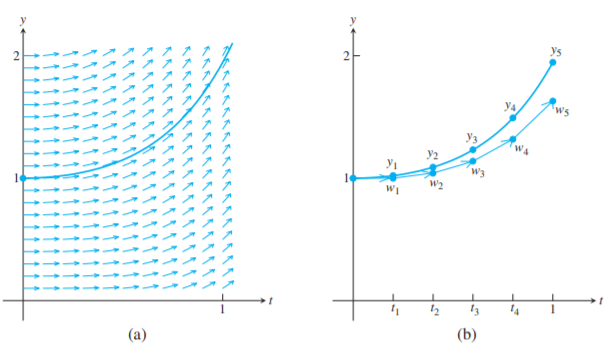
\includegraphics{rapport/metode/bilder/eulers.png}\newline\newline
Metoden innebærer å velge en startverdi for en kurve, for å så bevege seg en kort distanse langs denne. Så vil man re-evaluere kurven i det nye punktet og bevege seg en kort distanse langs denne. Slik fortsetter man til man får en tilnærmet løsning.\newline\newline
Kan da løse en likning $y' = f(t, y)$ ved å finne $w_i \approx y(t_i)$ gjennom å bruke følgende metode.
\begin{equation}
\begin{aligned}
    w_0&=y(t_0)\\
    w_{i+1}&=w_i + hf(t_i, w_i)
\end{aligned}
\end{equation}
I forbindelse med stive legemer ønsker man å bruke en variant av Eulers metode hvor $w_i$ er ortogonal. Bruker derfor en annen variant av Eulers metode hvor dette er mulig.
\begin{equation}
\begin{aligned}
    W_0&=X_0\\
    W_{i+1}&=W_iexp(h\Omega)
\end{aligned}
\end{equation}
Her angis startverdien $W_0=X_0$ som startposisjonen til det stive legeme, mens $W_iexp(h\Omega)$ returner en matrise som angir den nye posisjonen $W_{i+1}$.


\subsection{Midtpunkts-metoden}
\begin{center}
    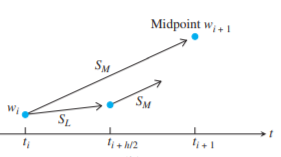
\includegraphics{rapport/metode/bilder/midpoint.PNG}
\end{center}
Midtpunkts-metoden tar utgangspunkt i Eulers metode. Forskjellen er at i midtpunkts-metoden finner man først midtpunktet mellom stegene, så beregner man tangenten til neste steg basert på midtpunktet.\newline\newline
Kan da løse en likning $y' = f(t, y)$ ved å finne $w_i \approx y(t_i)$ gjennom å bruke følgende metode.

\begin{equation}
\begin{aligned}
    w_0&=y(t_0)\\
    w_{i+1}&=w_i + hf(t_i+\frac{h}{2}, w_i+\frac{h}{2}f(t_i, w_i)
\end{aligned}
\end{equation}
Her ønsker vi også at $w_i$ skal være ortogonal, så vi tar utgangspunkt i den samme varianten av Eulers metode fra likning (12). Forskjellen er at vi beregner matrisen fra midtpunktet $i+\frac{1}{2}$.
\begin{equation}
\begin{aligned}
    W_0&=X_0\\
    W_{i+1}&=W_iexp(h\Omega_{i+\frac{1}{2}})
\end{aligned}
\end{equation}


\subsection{Trapes-metoden}
\begin{center}
    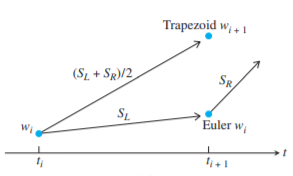
\includegraphics{rapport/metode/bilder/trapezoid.PNG}
\end{center}
Trapes-metoden tar også utgangspunkt i Eulers metode. Forskjellen her er at man regner ut tangenten i $w_i$, samt i $w_{i+1}$. Ved Trapes-metoden bruker vi da gjennomsnittet av disse tangentene. Dette illustreres i figuren overfor.\newline\newline
Kan da løse en likning $y' = f(t, y)$ ved å finne $w_i \approx y(t_i)$ gjennom å bruke følgende metode.

\begin{equation}
\begin{aligned}
    w_0&=y(t_0)\\
    w_{i+1}&=w_i + \frac{h}{2}(f(t_i, w_i)+f(t_{i+1}, w_{i+1}))
\end{aligned}
\end{equation}